\newpage
\section{Diagrammi dei packages}

\subsection{Introduzione}
Questa sezione racchiude i diagrammi dei packages, raccolti tramite un approccio top-down. Considerando l'approccio adottato, e il particolare applicativo realizzato con un pattern a Microservizi, non ci discosteremo dalla nomenclatura tradizionale di \textit{Classe} intesa come una categoria di entità in grado di svolgere uno specifico compito. Per mantenere una conformità con lo standard UML dunque, verrà utilizzato il termine \textit{classe} per indicare ciò che all'atto pratico sarà implementato come un microservizio vero e proprio, standalone, e con i propri metodi in grado di fornire la funzionalità preposta. Trattandosi di una progettazione con un livello di dettaglio intermedio, le classi non verranno definite, bensì verrà data una descrizione della loro funzionalità, lo scopo e le relazioni che intercorrono con le altre classi.

L'applicativo API Market è strutturato, come di consueto, in un lato Front-end ed un lato Back-end, come mostrato dal diagramma seguente:

\begin{figure}[H]
	\centering
	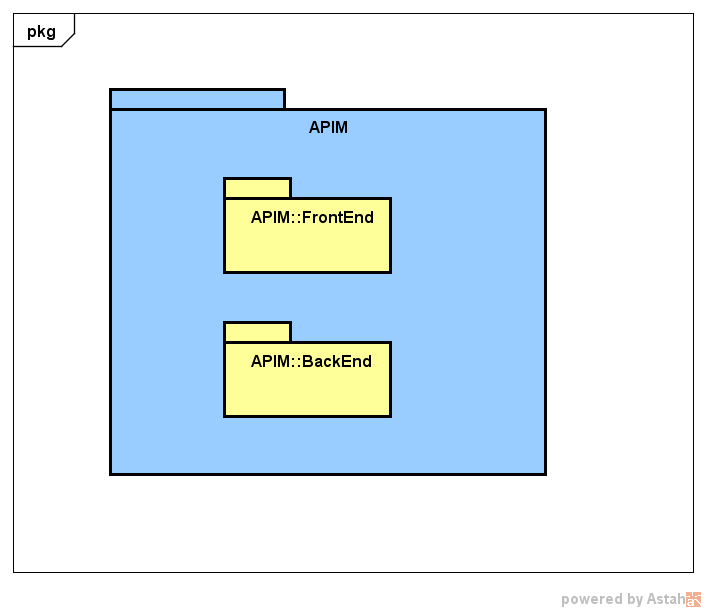
\includegraphics
	[width=0.7\linewidth]
	{UML/DiagrammiPackage/APIM.png}
	\caption{Package APIM}
\end{figure}

\subsection{Front-end}

Il lato Front-end risulta così strutturato:

\begin{figure}[H]
	\centering
	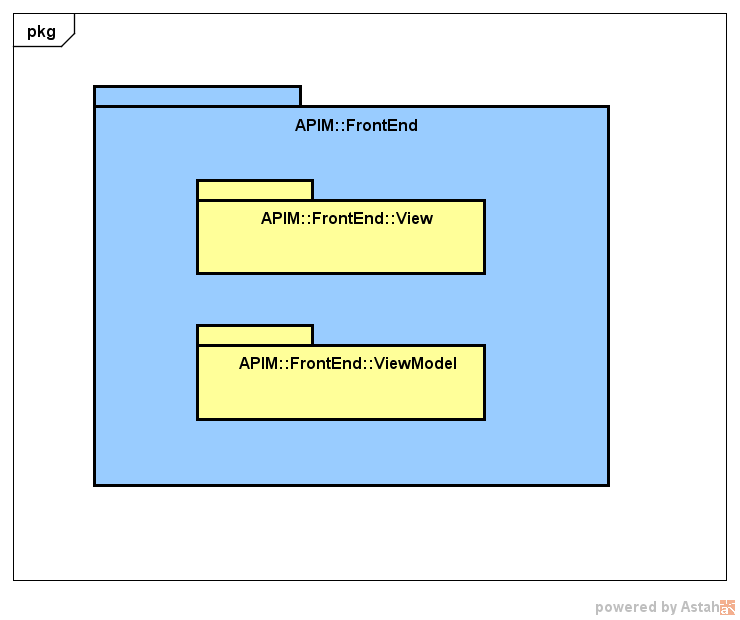
\includegraphics
	[width=0.7\linewidth]
	{UML/DiagrammiPackage/FrontEnd.png}
	\caption{Package APIM::FrontEnd}
\end{figure}

Nella parte Front-end sono dunque presenti i package View e ViewModel che rispecchiano l'architettura nativa dei framework da noi utilizzati.

\subsubsection{View}

Il package per il componente View contiene i seguenti sub-packages:

\begin{figure}[H]
	\centering
	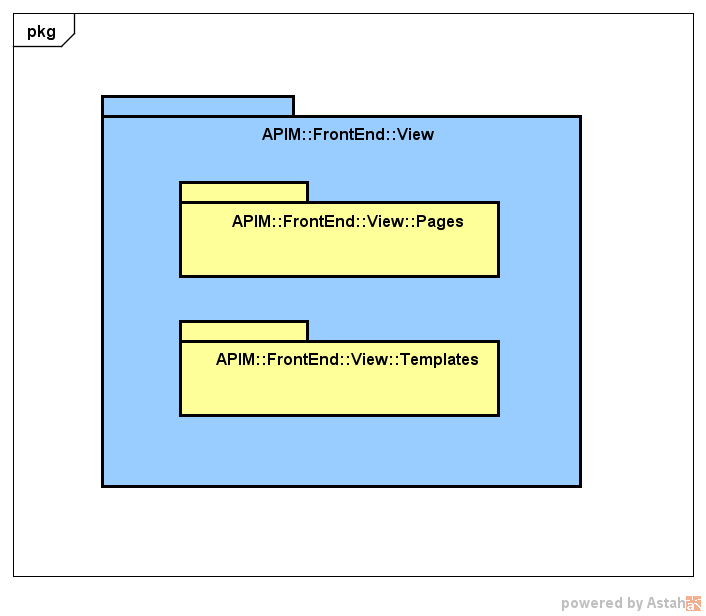
\includegraphics
	[width=0.7\linewidth]
	{UML/DiagrammiPackage/View.png}
	\caption{Package APIM::FrontEnd::View}
\end{figure}

\begin{itemize}
	\item \textbf{Pages}: Il package \textit{Pages} contiene una classe astratta \textit{Page}. Essa è poi utilizzabile tramite una derivazione concreta di tale classe, e l'implementazione avviene a seconda di ciò che è necessario visualizzare. Tali implementazioni possono usufruire dei template, per gestire situazioni standardizzate.
	\item \textbf{Templates}: Il package \textit{Templates} contiene un modello standard delle componenti utilizzabili per la rappresentazione. Ogni pagina che presenta situazioni e modelli analoghi può utilizzare un template già definito, per un maggior riuso, e per distinguere nettamente gli elementi contenuti in una pagina dalla loro realizzazione.
\end{itemize}

\subsubsection{ViewModel}

Il package per il componente ViewModel contiene i seguenti sub-packages:

\begin{figure}[H]
	\centering
	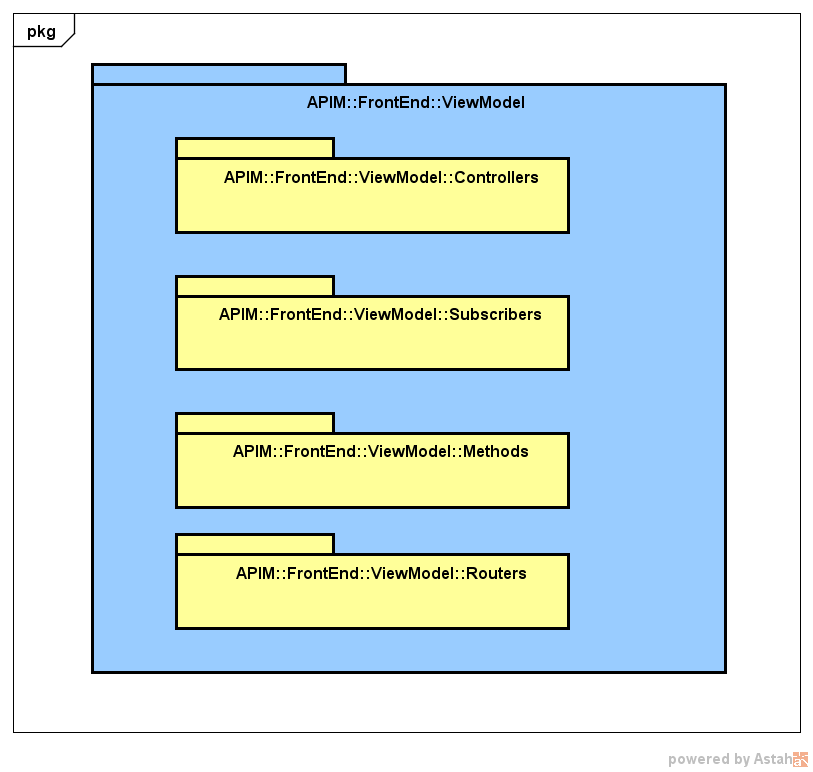
\includegraphics
	[width=0.7\linewidth]
	{UML/DiagrammiPackage/ViewModel.png}
	\caption{Package APIM::FrontEnd::ViewModel}
\end{figure}

La componente \textit{ViewModel} ha il compito di realizzare il data-binding con i componenti della \textit{View}, interagendo con la componente \textit{Model} che fornisce i dati o ne permette la modifica. La componente \textit{Model} è parte del lato Back-end della piattaforma, sebbene adottando un tale approccio si ha una linea di demarcazione meno netta tra le due parti. Di seguito si analizzano i packages contenuti all'interno del componente \textit{ViewModel}

\begin{itemize}
	\item \textbf{Controllers}: 
	\item \textbf{Subscribers}:
	\item \textbf{Methods}:
	\item \textbf{Routers}:
\end{itemize}
